\begin{refsection}

\chapter{Pb--Pb}
\label{ch:PbPb-R}

\noindent\begin{minipage}[t]{.3\linewidth}
\strut\vspace*{-\baselineskip}\newline
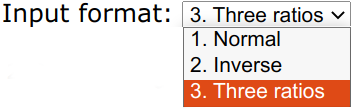
\includegraphics[width=\linewidth]{../figures/PbPbFormats.png}
\end{minipage}
\begin{minipage}[t]{.7\textwidth}
  \texttt{IsoplotR} accommodates three Pb--Pb formats. See
  Section~\ref{sec:PbPb} for details.
\end{minipage}

\begin{console}
PbPb <- read.data('PbPb.csv',method='Pb-Pb',format=3)
\end{console}

\noindent\begin{minipage}[t]{.15\linewidth}
\strut\vspace*{-\baselineskip}\newline
\includegraphics[width=\linewidth]{../figures/PbPbPlotdevices.png}\\
\end{minipage}
\begin{minipage}[t]{.85\textwidth}
  Pb--Pb data can be visualised on five different plot devices.
  Additionally, the single aliquot age estimates can also be reported
  in a downloadable data table.
\end{minipage}

\noindent\begin{minipage}[t]{.6\linewidth}
\strut\vspace*{-\baselineskip}\newline
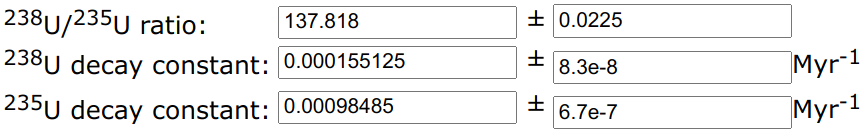
\includegraphics[width=\linewidth]{../figures/PbPbLambda.png}
\end{minipage}
\begin{minipage}[t]{.4\linewidth}
  The default \textsuperscript{238}U/\textsuperscript{235}U ratio is
  given by \citet{hiess2012}, and the U decay constants by
  \citet{jaffey1971}. These values can be changed here.
\end{minipage}

\begin{script}
# use the Steiger and Jaeger (1977) value with zero uncertainty
settings('iratio','U238U235',137.88,0)
# use the Schoene et al. (2006) value and uncertainty
settings('lambda','U238',0.000154993,0.00000013) 
\end{script}

\section{Isochrons}

\begin{enumerate}

\item \texttt{IsoplotR} offers three options to deal with the scatter of the
  data around the best-fit isochron line.

\noindent\begin{minipage}[t]{.45\linewidth}
\strut\vspace*{-\baselineskip}\newline
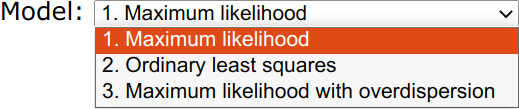
\includegraphics[width=\linewidth]{../figures/PbPbIsochronModels.png}
\end{minipage}
\begin{minipage}[t]{.55\linewidth}
  These three models represent three different ways to capture any
  excess dispersion of the data relative to the nominal uncertainties
  (Figure~\ref{fig:wtdmeanMSWD}).
\end{minipage}

\begin{console}
isochron(PbPb,model=1)
\end{console}

\item Data can be fitted using conventional
  (\textsuperscript{207}Pb/\textsuperscript{204}Pb
  vs. \textsuperscript{206}Pb/\textsuperscript{204}Pb) or
  (\textsuperscript{207}Pb/\textsuperscript{206}Pb
  vs. \textsuperscript{204}Pb/\textsuperscript{206}Pb) isochrons
  (Section~\ref{sec:inverseIsochrons}).

  \noindent\begin{minipage}[t]{.22\linewidth}
\strut\vspace*{-\baselineskip}\newline

\includegraphics[width=\linewidth]{../figures/PbPbisochronInverse.png}
\end{minipage}
\begin{minipage}[t]{.78\linewidth}
  These two types of isochron yield similar ages provided that the
  uncertainties are relatively small compared to the isotopic ratio
  values.
\end{minipage}

\begin{console}
isochron(PbPb,inverse=TRUE)
\end{console}

\item As discussed in Section~\ref{sec:SKgrowth}, the mantle evolution
  model of \citet{stacey1975} can be included with the isochron plot.
  Any intersection(s) of the isochron with the mantle evolution curve
  is/are reported in the plot legend.

\noindent\begin{minipage}[t]{.45\linewidth}
\strut\vspace*{-\baselineskip}\newline

\includegraphics[width=\linewidth]{../figures/PbPbIsochronSKcurve.png}
\end{minipage}
\begin{minipage}[t]{.55\linewidth}
  The Stacey-Kramers curve may not be easy to spot for very radiogenic
  samples.
\end{minipage}

\item The appearance and numerical behaviour of Pb--Pb isochrons can
  be modified using similar options as the U--Pb isochrons of
  Section~\ref{sec:UPb-isochron-R}.

\noindent\begin{minipage}[t]{.4\linewidth}
\strut\vspace*{-\baselineskip}\newline
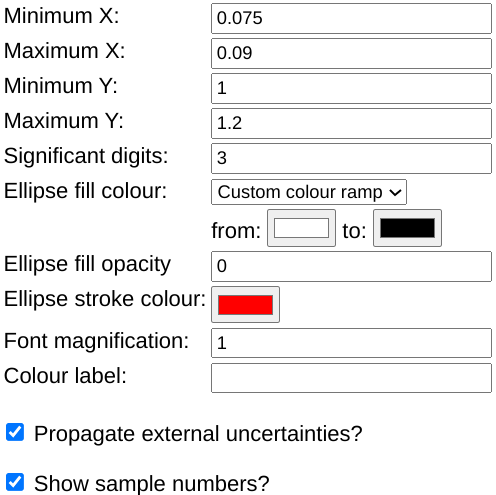
\includegraphics[width=\linewidth]{../figures/PbPbIsochronOtherOptions.png}
\end{minipage}
\begin{minipage}[t]{.6\linewidth}
  Tick the checkbox to propagate decay constant uncertainties
  (\texttt{exterr}) and label the error ellipses with the row numbers
  of the input data (\texttt{show.numbers}), use the textboxes to set
  the axis limits (\texttt{xlim} and \texttt{ylim}), significance
  level (\texttt{alpha}), significant digits (\texttt{sigdig}), the
  fill and stroke colour of the error ellipses (\texttt{ellipse.fill}
  and \texttt{ellipse.stroke}), font size (\texttt{cex}) and colour
  legend (\texttt{levels} and \texttt{clabel}).  
\end{minipage}

\begin{script}
isochron(PbPb,exterr=TRUE,show.numbers=TRUE,xlim=c(0,0.03),ylim=c(0,0.75),
         alpha=0.01,sigdig=3,ellipse.fill=NA,ellipse.stroke="red")
\end{script}
  
\end{enumerate}

\section{Radial plots}\label{sec:PbPbRadial}

\begin{enumerate}

\item The Pb--Pb method is usually applied to cogenetic aliquots that are
best analysed by isochron regression. The radial plot can serve a
useful purpose in visualising the residuals of the individual aliquots
around the best fit isochron line.\\

\noindent\begin{minipage}[t]{.35\linewidth}
\strut\vspace*{-\baselineskip}\newline
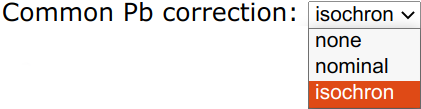
\includegraphics[width=\linewidth]{../figures/PbPbRadialPb0.png}
\end{minipage}
\begin{minipage}[t]{.65\linewidth}
  In contrast with the U--Pb data of Section~\ref{sec:UPbRadial}, the
  common Pb correction of Pb--Pb data is limited to two options:
  nominal and isochron. These implement the two procedures shown in
  Figure~\ref{fig:ThPbSingleGrain}.
\end{minipage}

\begin{console}
radialplot(PbPb,common.Pb=2)
\end{console}

\item Nominal common Pb correction proceeds like the nominal common Pb
  correction of U--Pb data formats 4--6 (Section~\ref{sec:general}).

\noindent\begin{minipage}[t]{.4\linewidth}
\strut\vspace*{-\baselineskip}\newline
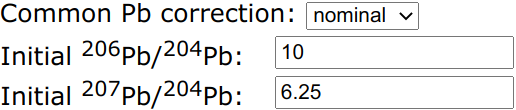
\includegraphics[width=\linewidth]{../figures/PbPbnominalPb0.png}
\end{minipage}
\begin{minipage}[t]{.6\linewidth}
  The nominal \textsuperscript{207}Pb/\textsuperscript{204}Pb and
  \textsuperscript{206}Pb/\textsuperscript{204}Pb ratios in this
  example correspond to a
  \textsuperscript{207}Pb/\textsuperscript{206}Pb ratio of 0.625,
  which equals the y-intercept of the inverse isochron.
\end{minipage}

\begin{console}
settings('iratio','Pb207Pb204',6.25)
settings('iratio','Pb206Pb204',10)
radialplot(PbPb,common.Pb=1)
\end{console}

\item After possible common Pb correction, the resulting Pb--Pb ages
  are treated in exactly the same way as the U--Pb data of
  Section~\ref{sec:UPbRadial}.

\noindent\begin{minipage}[t]{.3\linewidth}
\strut\vspace*{-\baselineskip}\newline
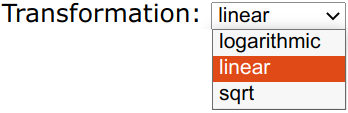
\includegraphics[width=\linewidth]{../figures/PbPbRadialTransformations.png}
\end{minipage}
\begin{minipage}[t]{.7\linewidth}
The data can be subjected to a linear, logarithmic or square root
transformation.
\end{minipage}

\begin{console}
radialplot(PbPb,transformation='linear')
\end{console}

\noindent\begin{minipage}[t]{.3\linewidth}
\strut\vspace*{-\baselineskip}\newline
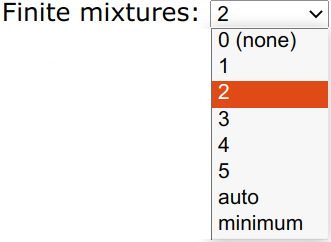
\includegraphics[width=\linewidth]{../figures/PbPbRadialMixtures.png}
\end{minipage}
\begin{minipage}[t]{.7\linewidth}
  The single grain ages can be subjected to finite mixture modelling
  with up to 5 components as well as the minimum age model.
\end{minipage}

\begin{console}
radialplot(PbPb,k=2)
\end{console}

\item All other properties of the radial plot are the same as for the
  U--Pb method:

\noindent\begin{minipage}[t]{.5\linewidth}
\strut\vspace*{-\baselineskip}\newline
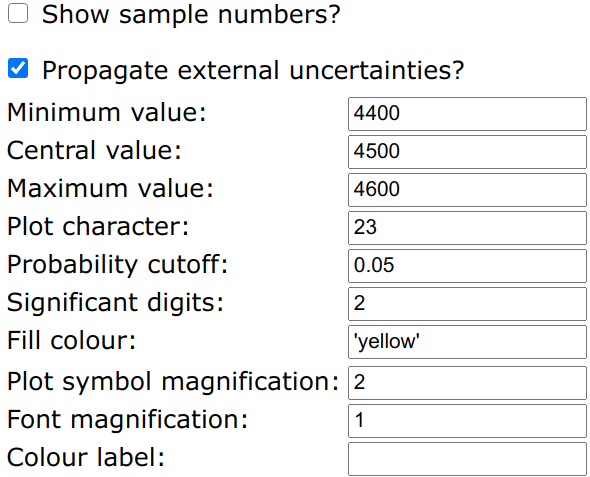
\includegraphics[width=\linewidth]{../figures/PbPbRadialOtherProperties.png}
\end{minipage}
\begin{minipage}[t]{.5\linewidth}
  The minimum and maximum extent of the radial scale can be specified,
  as well as the central value ($z_\circ$ in
  Equation~\ref{eq:radial}). Samples are represented by filled circles
  by default, but this can be changed to a range of other shape. These
  can be specified as numbers (\texttt{1-25}, see \texttt{?pch} for
  further details) or a single character such as \verb|'o'|,
  \verb|'*'|, \verb|'+'|, or \verb|'.'|. Plot characters that have a
    fill colour (e.g., \texttt{21-25}), an additional variable can be
    used to construct a colour scale. Both the plot symbols and any
    text labels in the plot of legend can be magnified or reduced via
    a scaling factor.
\end{minipage}

\begin{script}
radialplot(PbPb,from=4400,to=4600,t0=4500,
           pch=23,bg='yellow',cex=2,exterr=TRUE)
\end{script}

\end{enumerate}

\section{Weighted mean}\label{sec:PbPbWtdMean}

Following possible common Pb correction, the weighted mean function
for the Pb--Pb method works in exactly the same way as for the U--Pb
method.\\

\noindent\begin{minipage}[t]{.4\linewidth}
\strut\vspace*{-\baselineskip}\newline
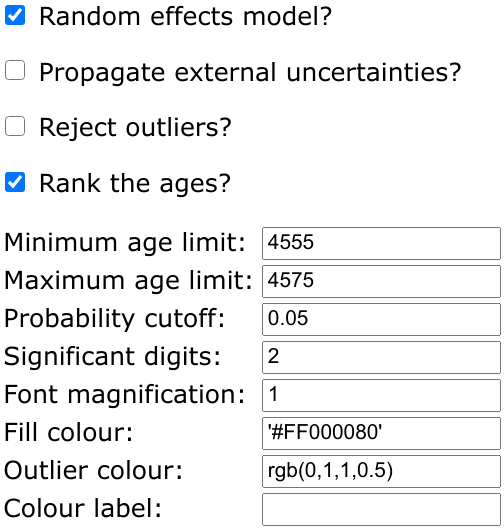
\includegraphics[width=\linewidth]{../figures/PbPbWeightedMeanOptions.png}
\end{minipage}
\begin{minipage}[t]{.6\linewidth}
  Tick the box to use the two parameter random effects model of
  Equation~\ref{eq:wtdmean-model-3} (\texttt{random.effects}),
  propagate decay constant uncertainties (\texttt{exterr}), reject
  outliers (\texttt{detect.outliers}), or rank the aliquots in
  increasing age (\texttt{ranked}). Use the textboxes to specify the
  minimum (\texttt{from}) and maximum (\texttt{to}) extent of the time
  axis, the significance levels of the error bars and confidence
  intervals (\texttt{alpha}), the number of significant digits used in
  the legend (\texttt{sigdig}), the font of the text in the figure
  labels and legend (\texttt{cex}), the background colour of the
  sample boxes for the regular aliquots (\texttt{bg}) and outliers
  (\texttt{outlier.col}) and the label of any possible colour legend
  (\texttt{levels} and \texttt{clabel}).
\end{minipage}

\begin{script}
weightedmean(PbPb,random.effects=TRUE,exterr=FALSE,detect.outliers=FALSE,
             ranked=TRUE,from=4555,to=4575,bg='#FF000080')
\end{script}

\section{Ages}\label{sec:PbPbAges}

\printbibliography[heading=subbibliography]

\end{refsection}
